\chapter{Modeling human representational geometry}
\label{chap:modeling_human}

From a historical point of view, the success of RSA brought to many studies on ablation, plasticity, etc. Many researchers used it, but they started questioning whether it is a good model of human knowledge. In the following we are discussing different assumptions, in respect to artificial DNN.

\subsection{Background}
We have already seen in Chapter \ref{chap:concepts_categories} the most accepted representation of concepts, as categories, in psychology: semantic domains or categories (e.g. mammals, animals, dogs) are organized via features or dimensions that carry the relevant variance for the category (Classical view, Rosch and Mervis (1975), \cite{lake-2015-deep}).
We have also seen how we can have typicality effects in AI: entities (e.g. images, words) are described by feature values from which representational category effects emerge.\\

We can use AI systems as models of semantics (Section \ref{sec:kriegeskorte}): AI systems trained for image categorization or word embedding produce representations that reasonably approximate those of humans. Similarity between categories, as operationalized from human data, is well predicted by distances between objects in the AI model, where human similarity is quantified using brain/behavior and model similarity is quantified via Euclidean distances, inverse cosine, etc.
For prediction of human similarity judgments on images, they found 20 to 60\% of the judgments is modeled by the NN. While in MVPA the results are more complicated: these can predict activation in brain areas, but the correlation is just barely above the significance threshold.

\subsection{AI modeling of human representations}
Modeling human representations with AI is useful for many fields:
\begin{itemize}
    \item Psychology: AI models achieve human-like competence on different tasks. Because of their competence, they offer a \textbf{model of potential knowledge organization}. They can also offer \textbf{interpretability of human behaviour}: if we have an AI model that behaves as humans, we can study it to come up with valid hypotheses.
    \item Engineering: better prediction of human behavior, and improved AI-human alignment. For instance, to evaluate how good generated images are, similarity metrics are used. However this does not take into account the subjectivity of human brain.
    \item Computer science: understanding representations in neural networks.
\end{itemize}

There are three approaches:
\begin{itemize}
    \item \textbf{Default}: \textbf{use all DNN features} (all in the whole network, or all in a particular layer) as object-representation for modeling human data. This implicitly assumes that all features are relevant and equally important, for the alignment, for all concepts.
    \item \textbf{Reweighting}: \textbf{keep all features, but adjust the weights by finetuning}. It addresses mis-calibrated, human-relevant features by applying concept-specific adjustment of feature saliency for modeling human representations. This assumes that AI learns human-relevant features, but these are mis-calibrated.
    \item \textbf{Pruning}: \textbf{keep the weights unchanged but remove some features}, investigating modular structures in AI models. This assumes that the network develops a modular structure where information about different categories is represented in different subspaces (subsets of latent dimensions) within the model, i.e., knowledge about particular categories or concepts is stored in particular areas (``modules") in the AI model.
\end{itemize}

\subsubsection{Default approach}
Assuming two objects, $U$ and $V$, each with 3 features, \textbf{human similarity} can be defined using the \textbf{inner product} (or a related quantity), and approximated as follows:
\[
    Similarity(V,U) = V \cdot U = V_1 \cdot U_1 +  V_2 \cdot U_2 + V_3 \cdot U_3
\]
Note this is just an evaluation (no learning involved).

\subsubsection{Reweighting approach, \cite{peterson}}
The similarity is defined as the \textbf{weighted inner product} (or related measure), where the weights ($W_{1,2,3}$) are learned via regression and evaluated on out-of-sample data.
\[
    Similarity(V,U) = W_1 \cdot V_1 \cdot U_1 + W_2 \cdot V_2 \cdot U_2 + W_3 \cdot V_3 \cdot U_3
\]
This \textbf{involves learning} (via linear regression or other techniques). Learning the weights is far from easy, since the number of free parameters is extremely huge (regularization is needed), as weight solutions are category-specific.

\cite{peterson} proved that this approach generalizes well, outperforming the baseline (default approach), despite this being already high.

\subsubsection{Pruning}
It aims at identifying a \textbf{subset of features}, \textbf{per category}, improving prediction of human representations, e.g.:
\[
    Similarity(V,U) = V_2 \cdot U_2 + V_3 \cdot U_3
\]
Pruning aims to find a subset of features that produces object-to-object distances that best match those produced from human behavior. By iterating over features and using \textit{Sequential Feature Selection} algorithms, supervised pruning learns a subset of features that \textbf{better predicts human judgments and generalizes to out-of-sample data}. It is supervised pruning since we are using human similarity judgments to choose which features to prune.

\boxc{Pruning at work: a toy example}{
Humans find Tigers more similar to Lions than to Pumas. The model representation is disaligned from human representation (as Tiger-Lion and Tiger-Puma distances are the same in the embedding space of the model).
We see that removing Y-Dimension brings the embedding space closer to human representation:
\begin{center}
    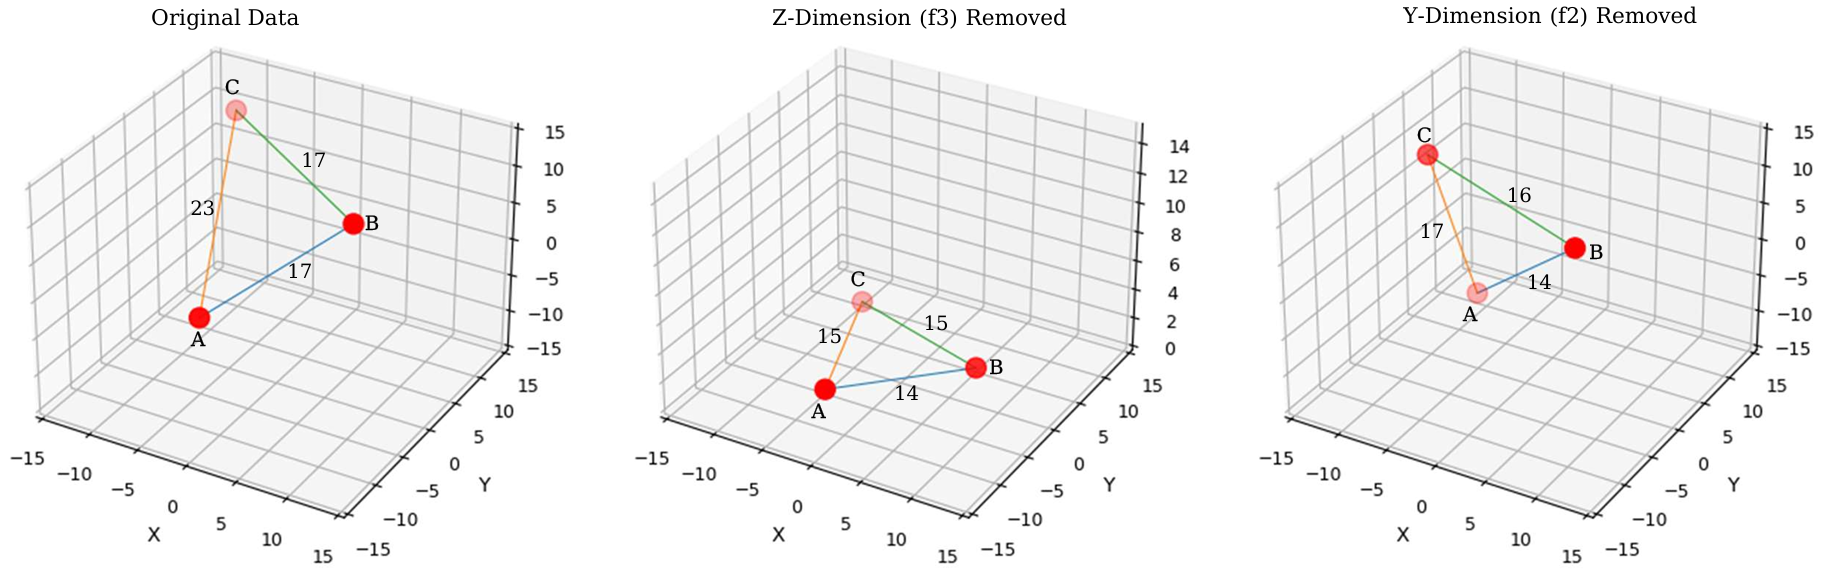
\includegraphics[width=0.9\textwidth]{images/pruning.png}
\end{center}
}
To summarize, pruning:
\begin{itemize}
    \item improves out-of-sample prediction accuracy for human similarity judgments of images, (higher RSA isomorphism);
    \item produces a more psychologically valid representational space;
    \item improves prediction of out-of-sample MVPA data (Brain RDMs).
\end{itemize}
Moreover, the feature-sets retained by pruning vary depending on the category guiding the pruning process, and these sets identify different subspaces (latent factors) in the feature space.
Pruning improves out of sample prediction of human similarity judgments for words and allows an interpretation of latent dimensions underlying word similarity judgments.

\boxl{\cite{TARIGOPULA202389}\\ \textit{Improved prediction of behavioral and neural similarity spaces using pruned DNNs}}{
They prune of a model that learns to predict human similarity judgments within 6 categories, each consisting of 120 images. In particular, they prune the penultimate layer of VGG19, which has 4096 nodes (features), and show that pruning outperforms other methods, including reweighting:
\begin{center}
    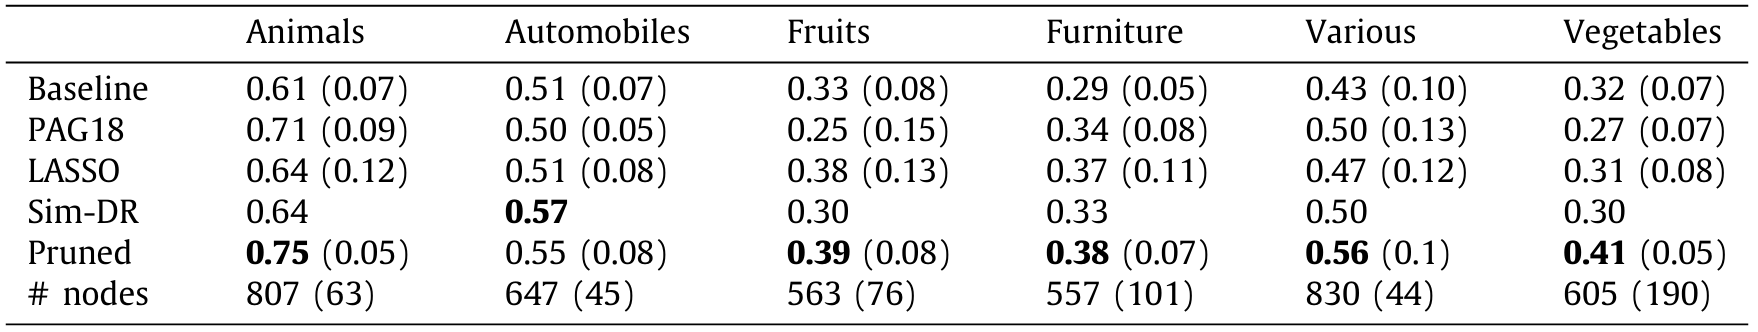
\includegraphics[width=0.8\textwidth]{images/tarigopula.png}
\end{center}
The number of nodes refers to how many nodes are retained by the pruning algorithm (e.g. for Animals 807 out of the original 4096).\\

They then proceed showing how pruning improves representational space for \textbf{out-of-sample image embeddings}. They first use a \textbf{different dataset} of Animal images and apply MDS (MultiDimentional Scaling); then they repeat but using only feature indices retained from pruning against the original experimental Animals dataset. In this second case, the animal types are better separated in the MDS representation (better clustering).

\begin{center}
    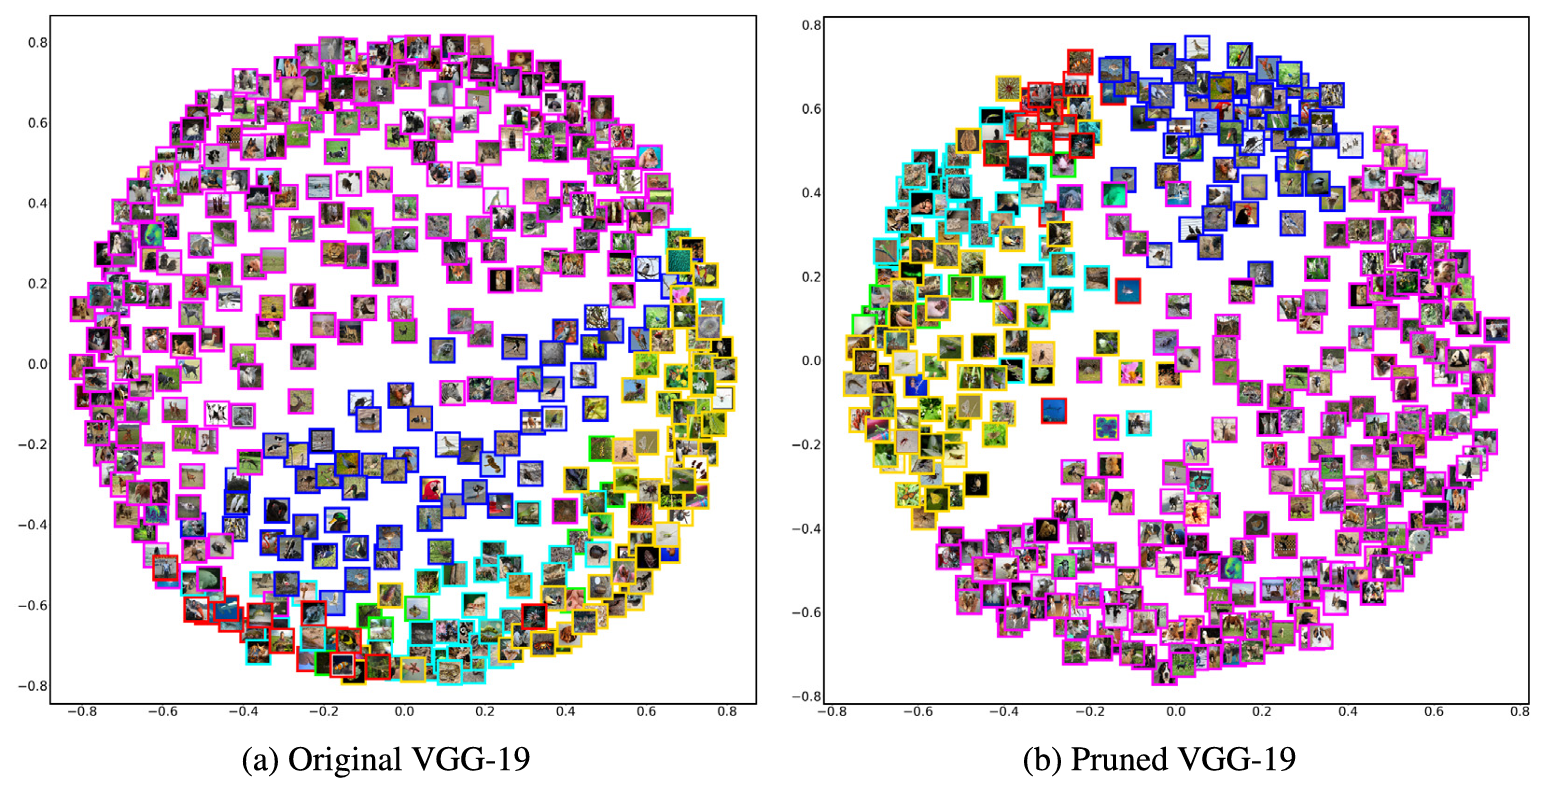
\includegraphics[width=0.7\textwidth]{images/mds.png}
\end{center}

Pruning also improves representational space for \textbf{out-of-sample brain data}. They use a dataset with two independent sets of 144 images. They produce RDMs from brain activity, per regions, then use RDMs to supervise pruning, and test on out-of-sample data, finding the prediction of brain-derived RDMs is improved.
}

\boxl{Bavaresco et al. (unpublished)\\ \textit{Continuation of \cite{TARIGOPULA202389}}}{
They try to understand whether the different feature sets retained by pruning, for each class, are similar; and whether they code for different information. To measure the overlap between the (indices of the) features retained from the different category they use the Dice-Sørensen coefficient:
\[
    DSC = 2 \cdot \frac{intersection}{union} 
\]
They find the lowest value for $\langle Fruits,Automobiles\rangle$ (0.13) and the highest for $\langle Fruits,Vegetables\rangle$ (0.28). It is not surprising that the highest DSC value is between fruits and vegetables, which are indeed similar. However, in general, the overlap is quite low.
They find that just 1 out of 4096 feature is always selected for all 6 categories, meaning that there is not a ``core" set of features that is always retained.\\

To know if the selected features identify different information, they use a different dataset of 50k images. \textbf{Images are represented using only activations on the retained features} (6 different versions: 50k$\times807$; 50k$\times647$, etc.). For each of these derived embeddings they \textbf{identified the top-5 images that maximize activation on that set of features} (i.e., highest sum by row (in the matrix with inputs in rows and features in columns). They find that pruning-retained features, per category, are \textbf{maximized by images that 
exemplify the category}. This is consistent with the prototype theory.\\

To have a more quantitative analysis, they apply PCA to each version (of the 6) and obtain the scores for the 50k images on the first Principal Component (this is needed since  the matrices are too large). Then the 50k PC1 scores are correlated across solutions (they get a score for each image). They conclude that \textbf{different retained sets select for different latent dimensions} (i.e., PC1 of similar categories encode for similar information).
}

\boxl{Manrique et al. (2023)\\ \textit{?}}{?}
